\subsection{25 августа. Д.р. Кичкинекол}
\textit{Метеоусловия: утром, днём тепло, переменная облачность; после 17:00 дождь с грозой}

\begin{figure}[h!]
	\centering
	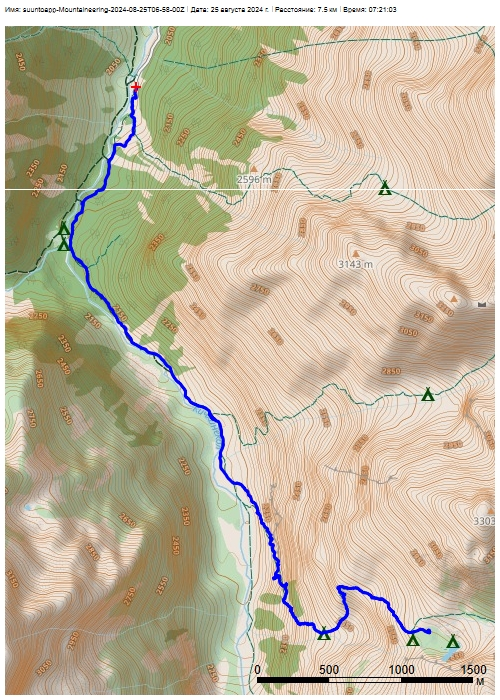
\includegraphics[angle=0, width=0.7\linewidth]{../pics/mini_maps/25}
	\label{fig:mini_25}
\end{figure}

Подъём в 6:30. Облачно, без осадков. Перепаковались (рис.~\ref{fig:DSC_0126.JPG}), оставили некоторые вещи и продукты сходящему участнику группы (Наташе). 

\begin{figure}[h!]
	\centering
	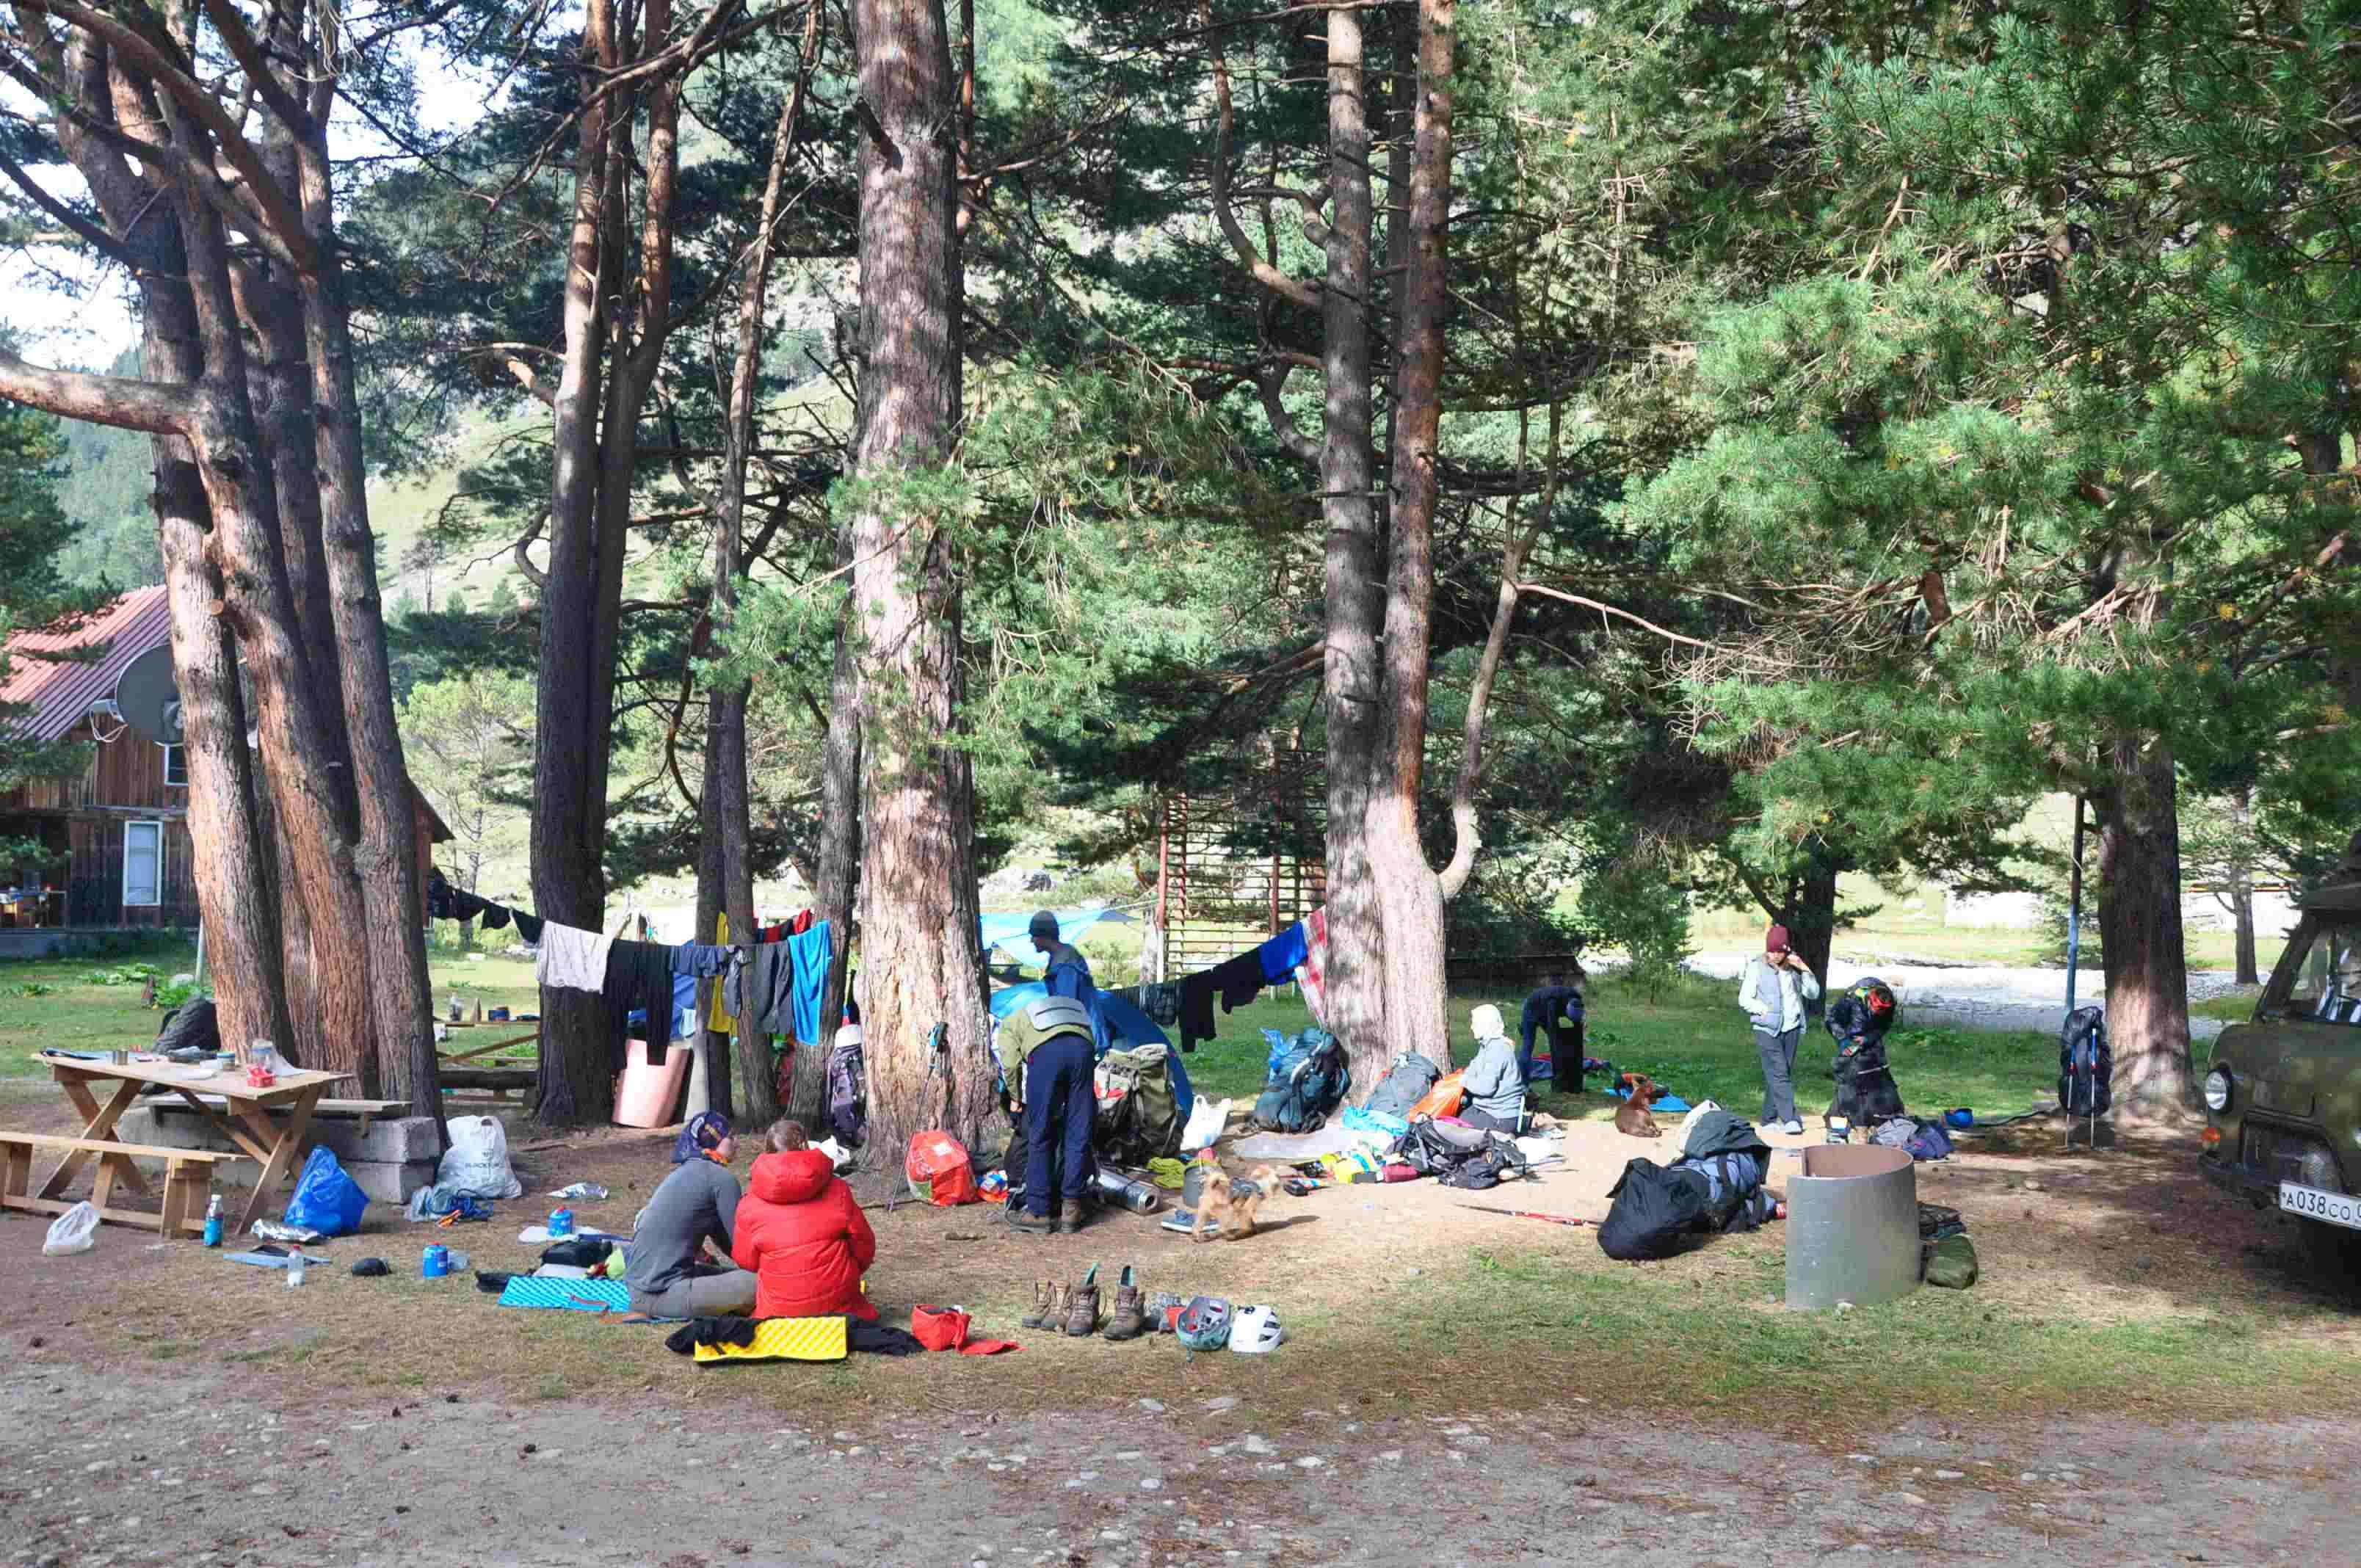
\includegraphics[width=0.7\linewidth]{../pics/DSC_0126.JPG}
	\caption{Утренние сборы в а/л <<Узункол>>}
	\label{fig:DSC_0126.JPG}
\end{figure}

Вышли в 9:58 по левому берегу р. Узункол. В 10:45 оказались в ущелье р. Кичкинекол (рис.~\ref{fig:DSC_0127.JPG}). 

\begin{figure}[h!]
	\centering
	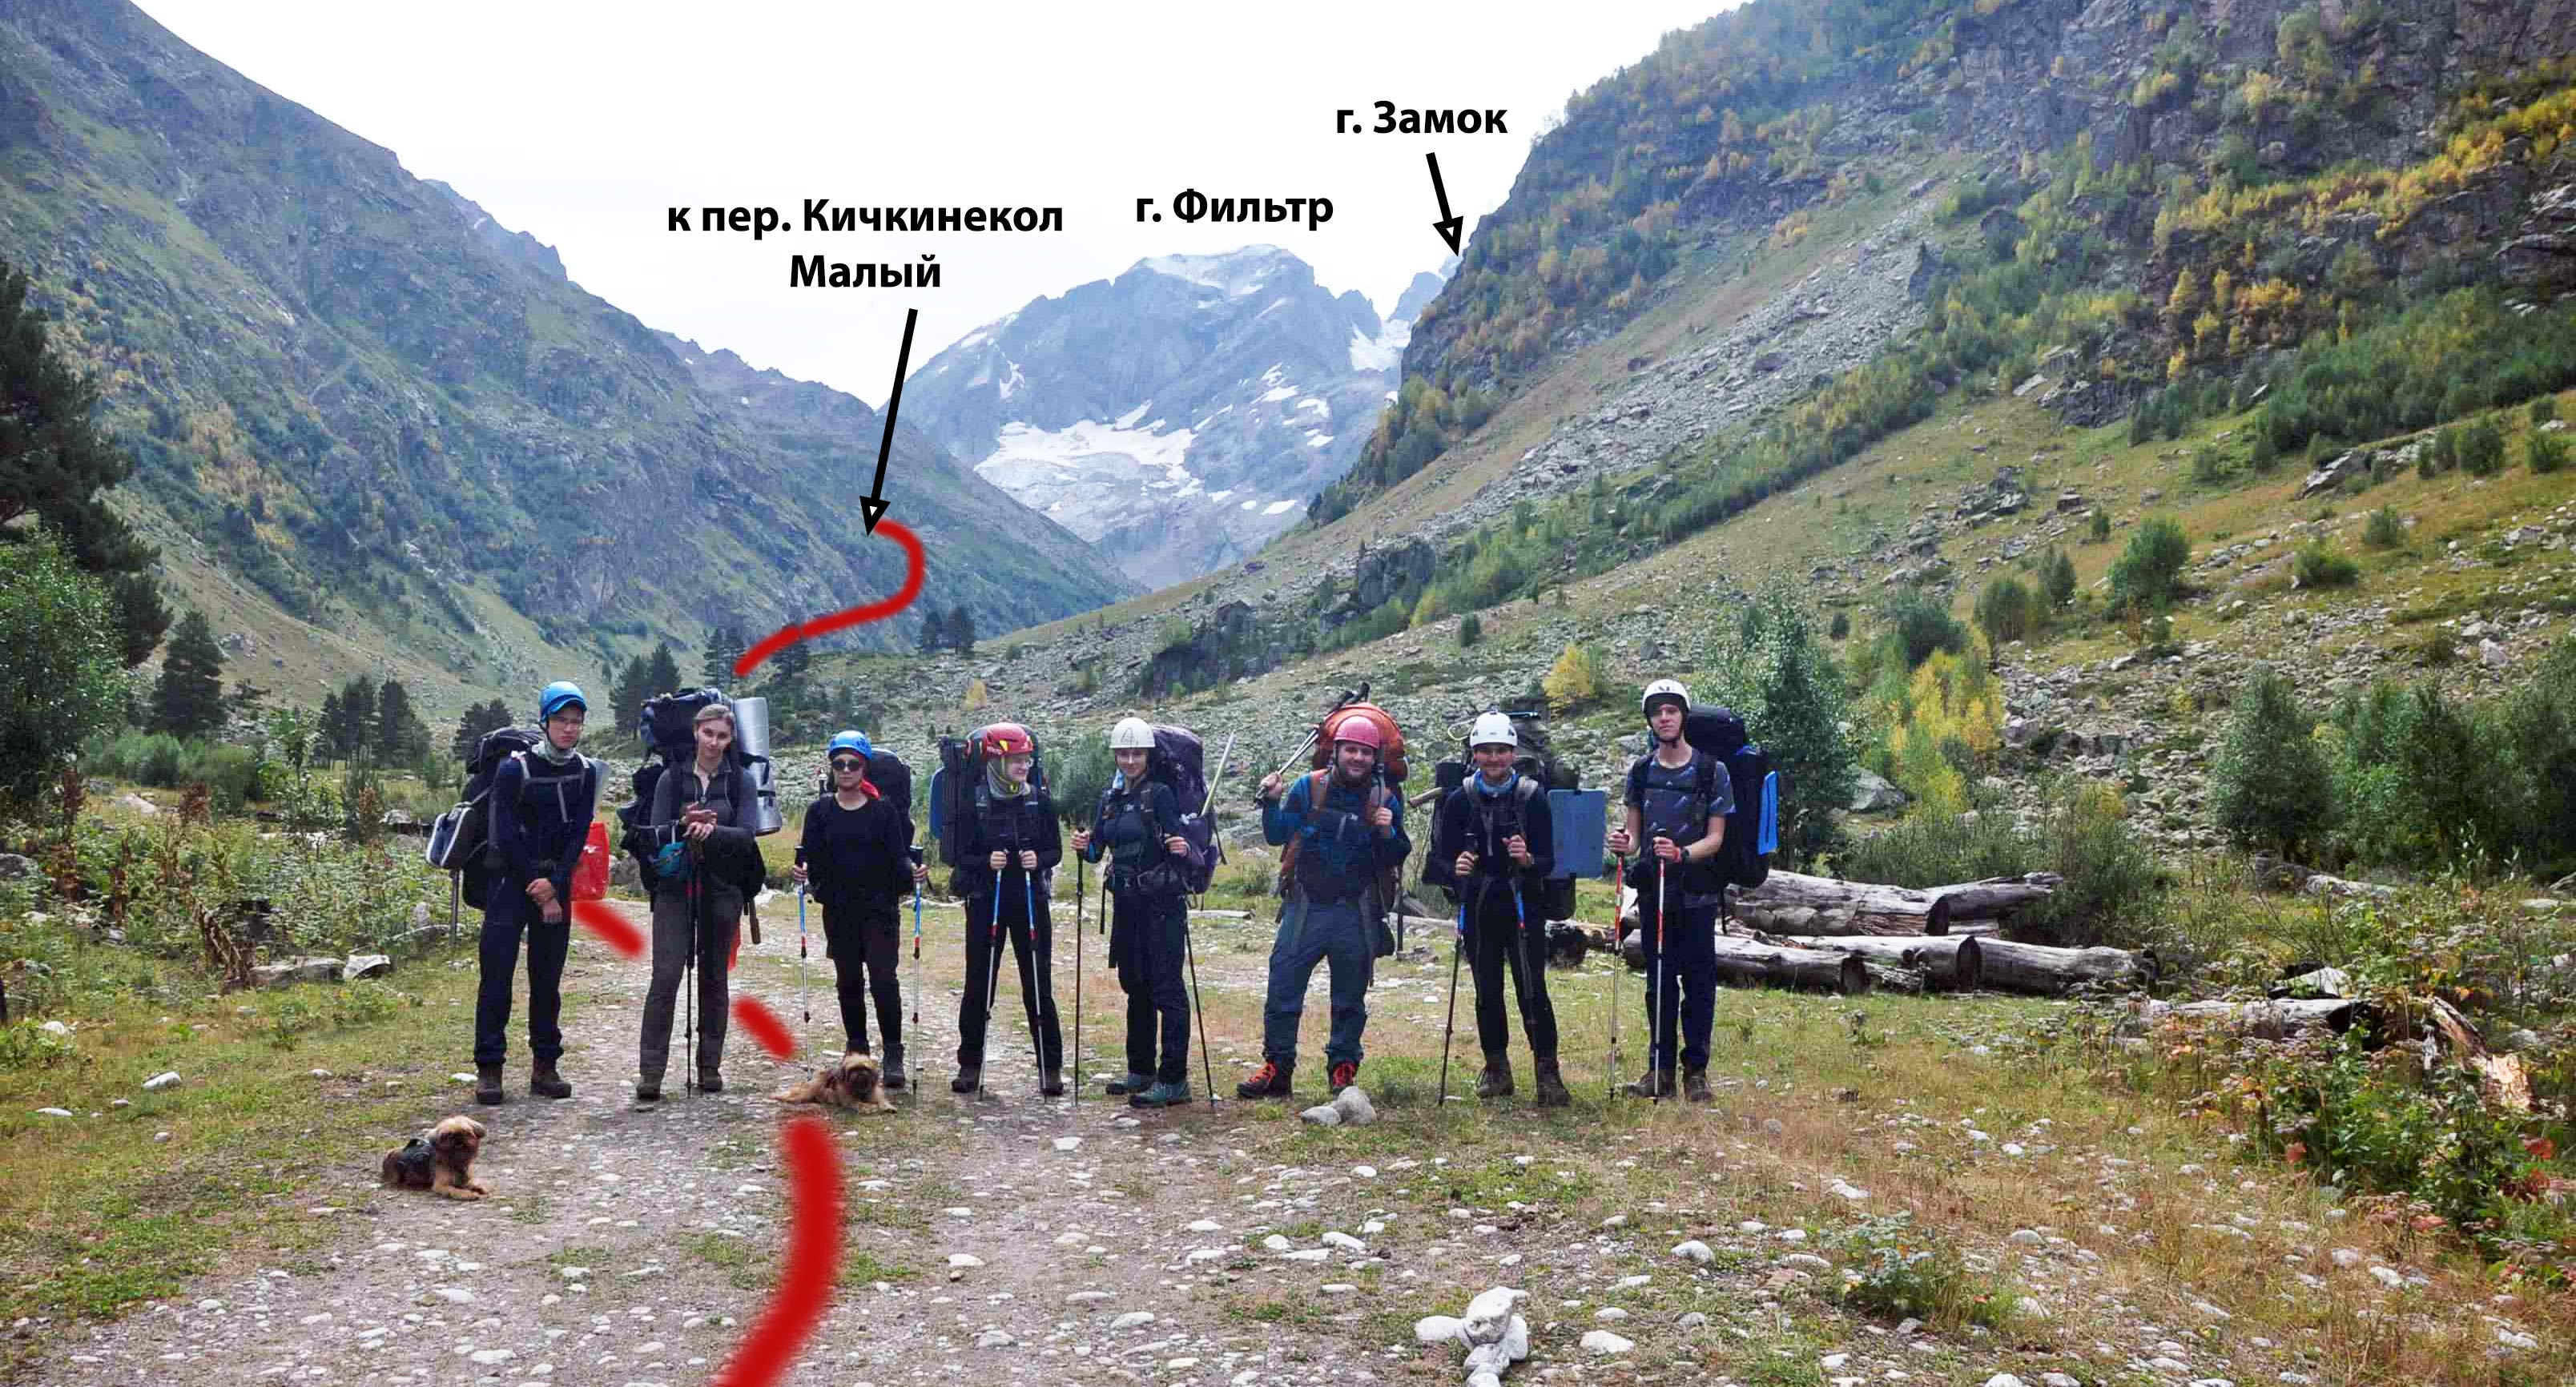
\includegraphics[width=0.7\linewidth]{../pics/DSC_0127.jpg}
	\caption{группа в ущелье р. Кичкинекол}
	\label{fig:DSC_0127.JPG}
\end{figure}


По ущелью идёт укатанная грунтовка, и мимо нас, пока мы шли, регулярно проезжали машины. В 11:12 прошли поворот на пер. Доломиты Южный (1А). Руководитель помнил, что группа Королёва \cite{Korolyov2018} в своё время пропустила тропу, ведущую косым траверсом в д.~р. Кичкинекол к нашему перевалу Кичкинекол Малый, и им пришлось подниматься в лоб по зарослям рододендронов, --- поэтому тропу стремились засечь как можно раньше и, боясь её пропустить, забрались на склон, как оказалось потом, слишком рано, за 200 м до начала тропы. Тем не менее, в 11:50 мы всё-таки подсекли искомую хорошо набитую тропу и продолжили движение по ней. (рис~\ref{fig:IMG_20240825_134744.jpg}).  
	
	\begin{figure}[h!]
		\centering
		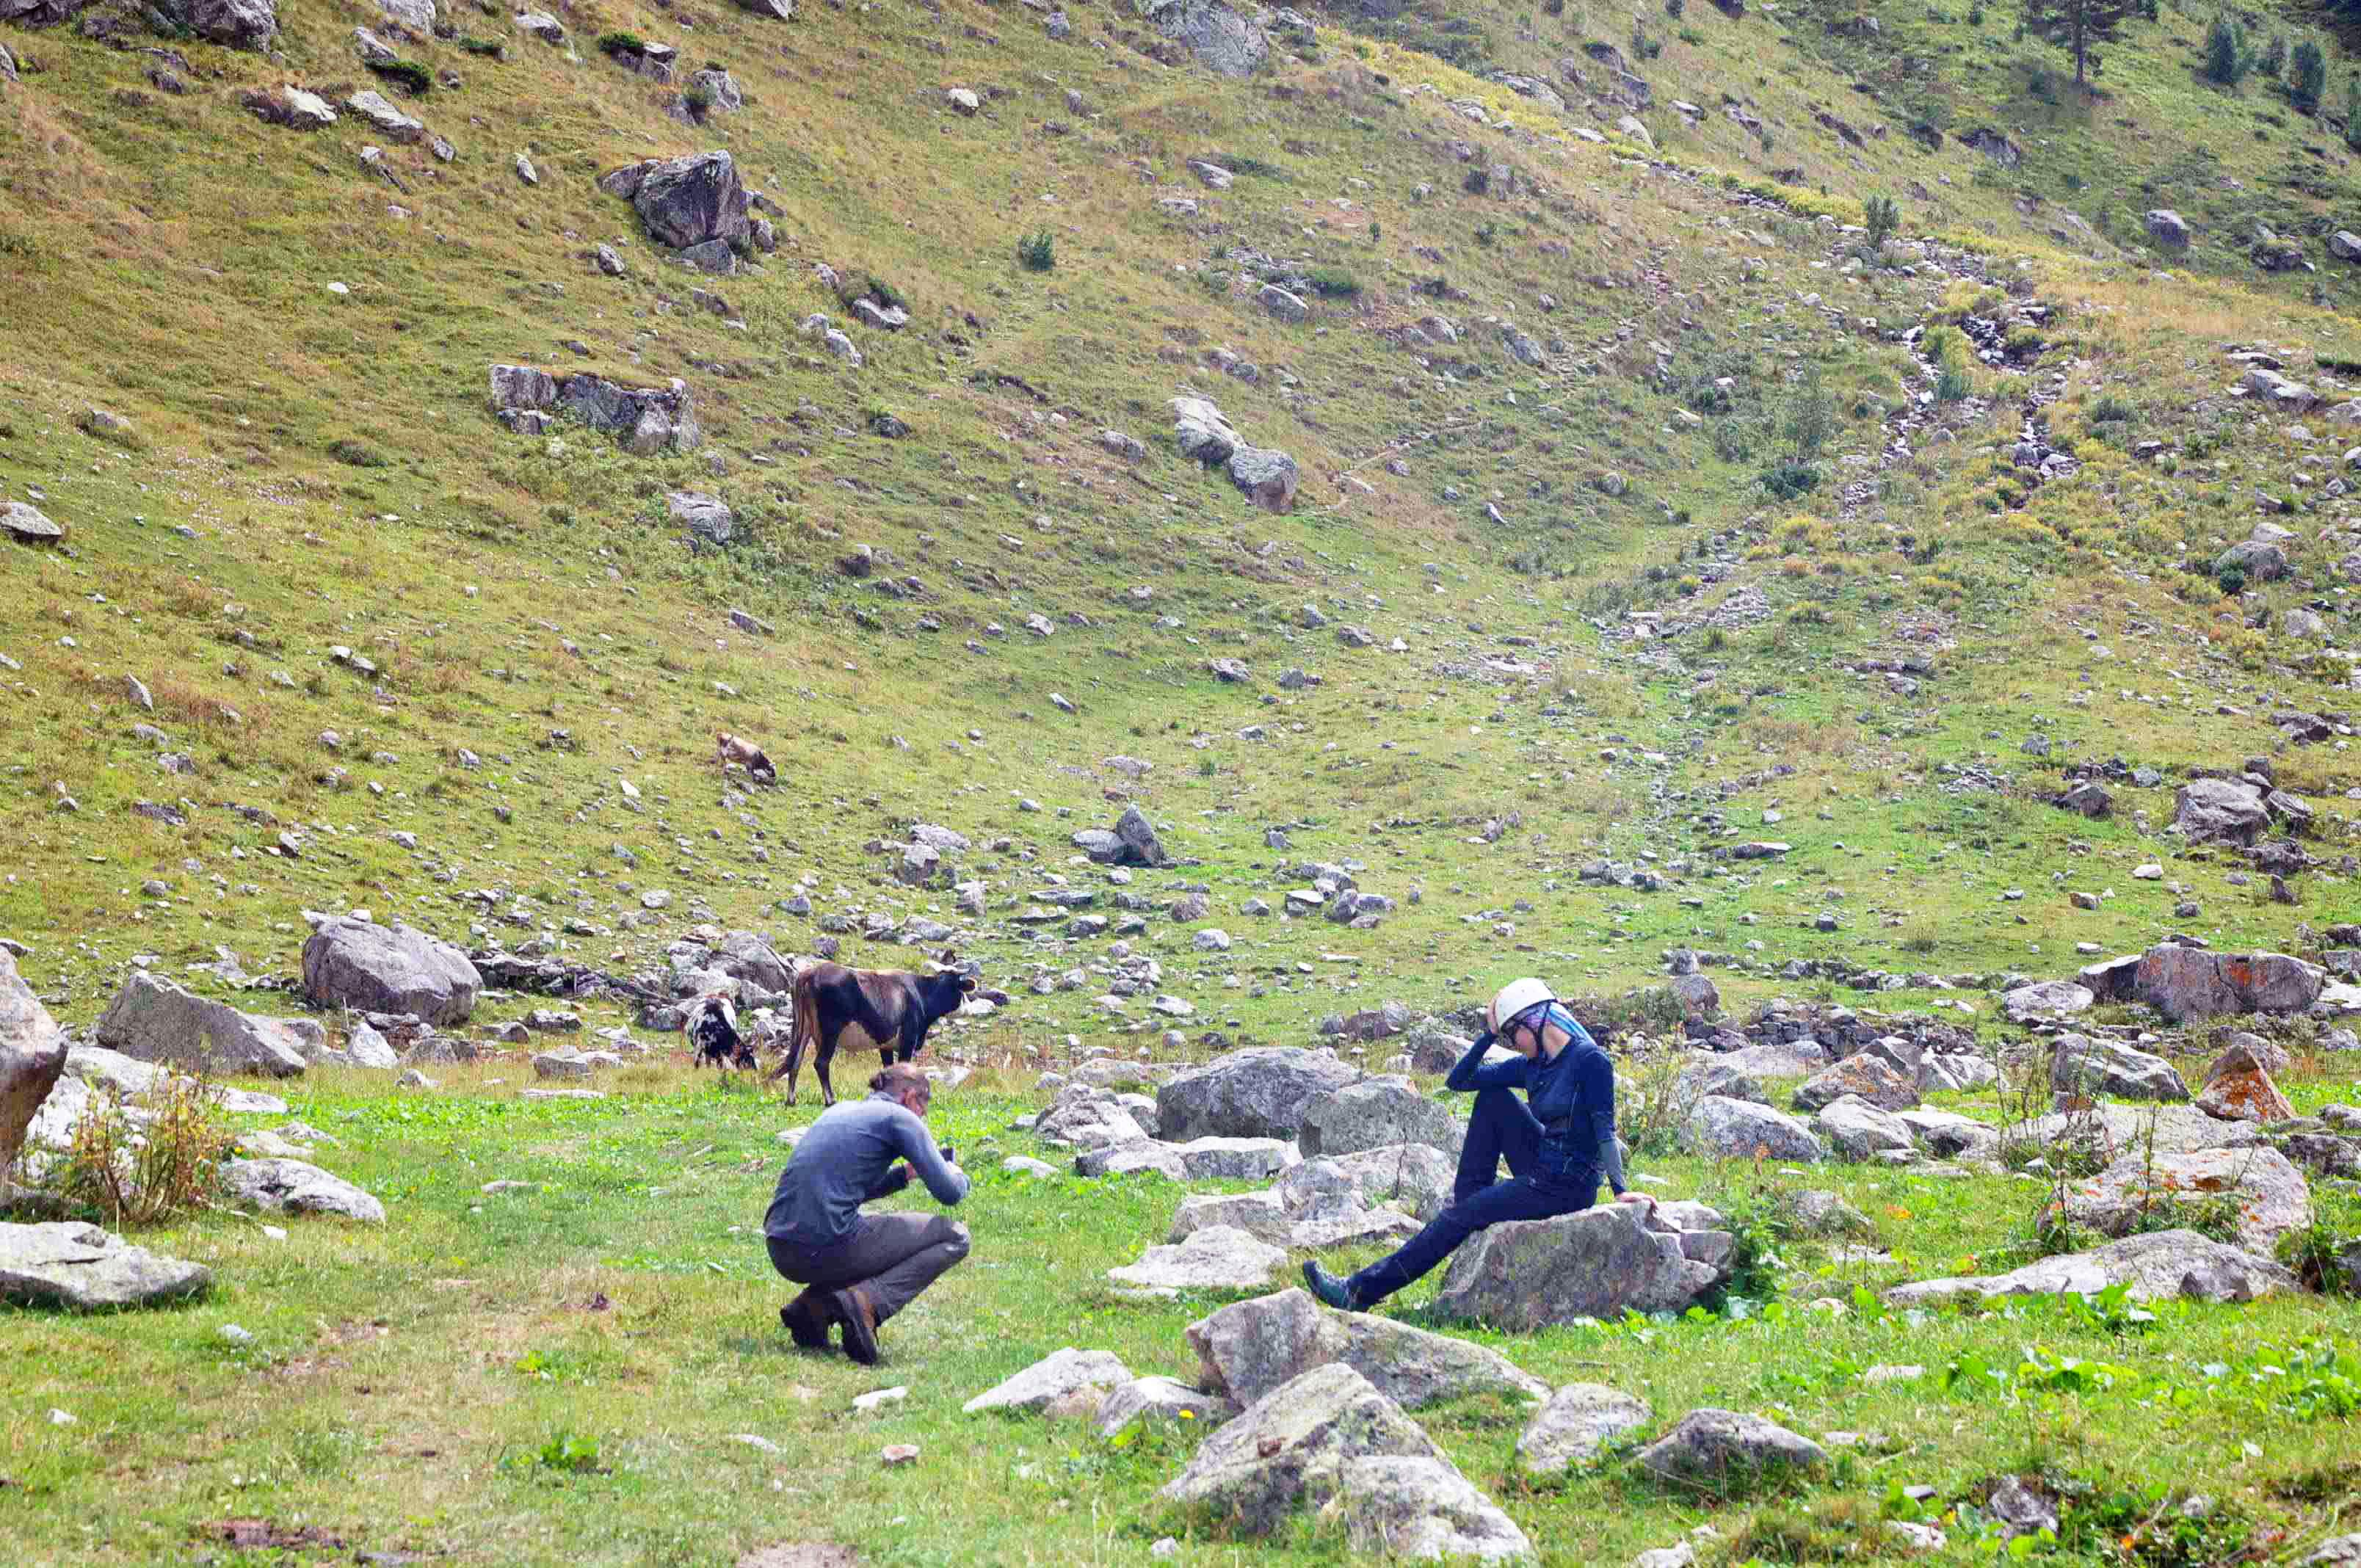
\includegraphics[width=0.7\linewidth]{../pics/DSC_0138.jpg}
		\caption{Начало подъёма на косогор в д.р. Таллычат}
		\label{fig:DSC_0138.JPG}
	\end{figure}
	
Возле водопада, на высоте 2365~м, в 13:06 сделали привал, чтобы набрать воды; вдобавок, руководитель понял, что на предыдущем привале оставил блокнот со своей любимой ручкой и карандашом и бинокль, и возвращался в попытке их найти --- к сожалению, безуспешно. Пришлось двигаться дальше. (Если кто-нибудь найдёт блокнот, бинокль и ручку --- сообщите, пожалуйста!) Идя по тропе, набирали высоту по графику 15/10 минут. Погода была всё ещё пасмурной, но движению ничего не мешало. Мест для обеда не было, поэтому питались карманкой и сухим пайком.

\begin{figure}[h!]
	\centering
	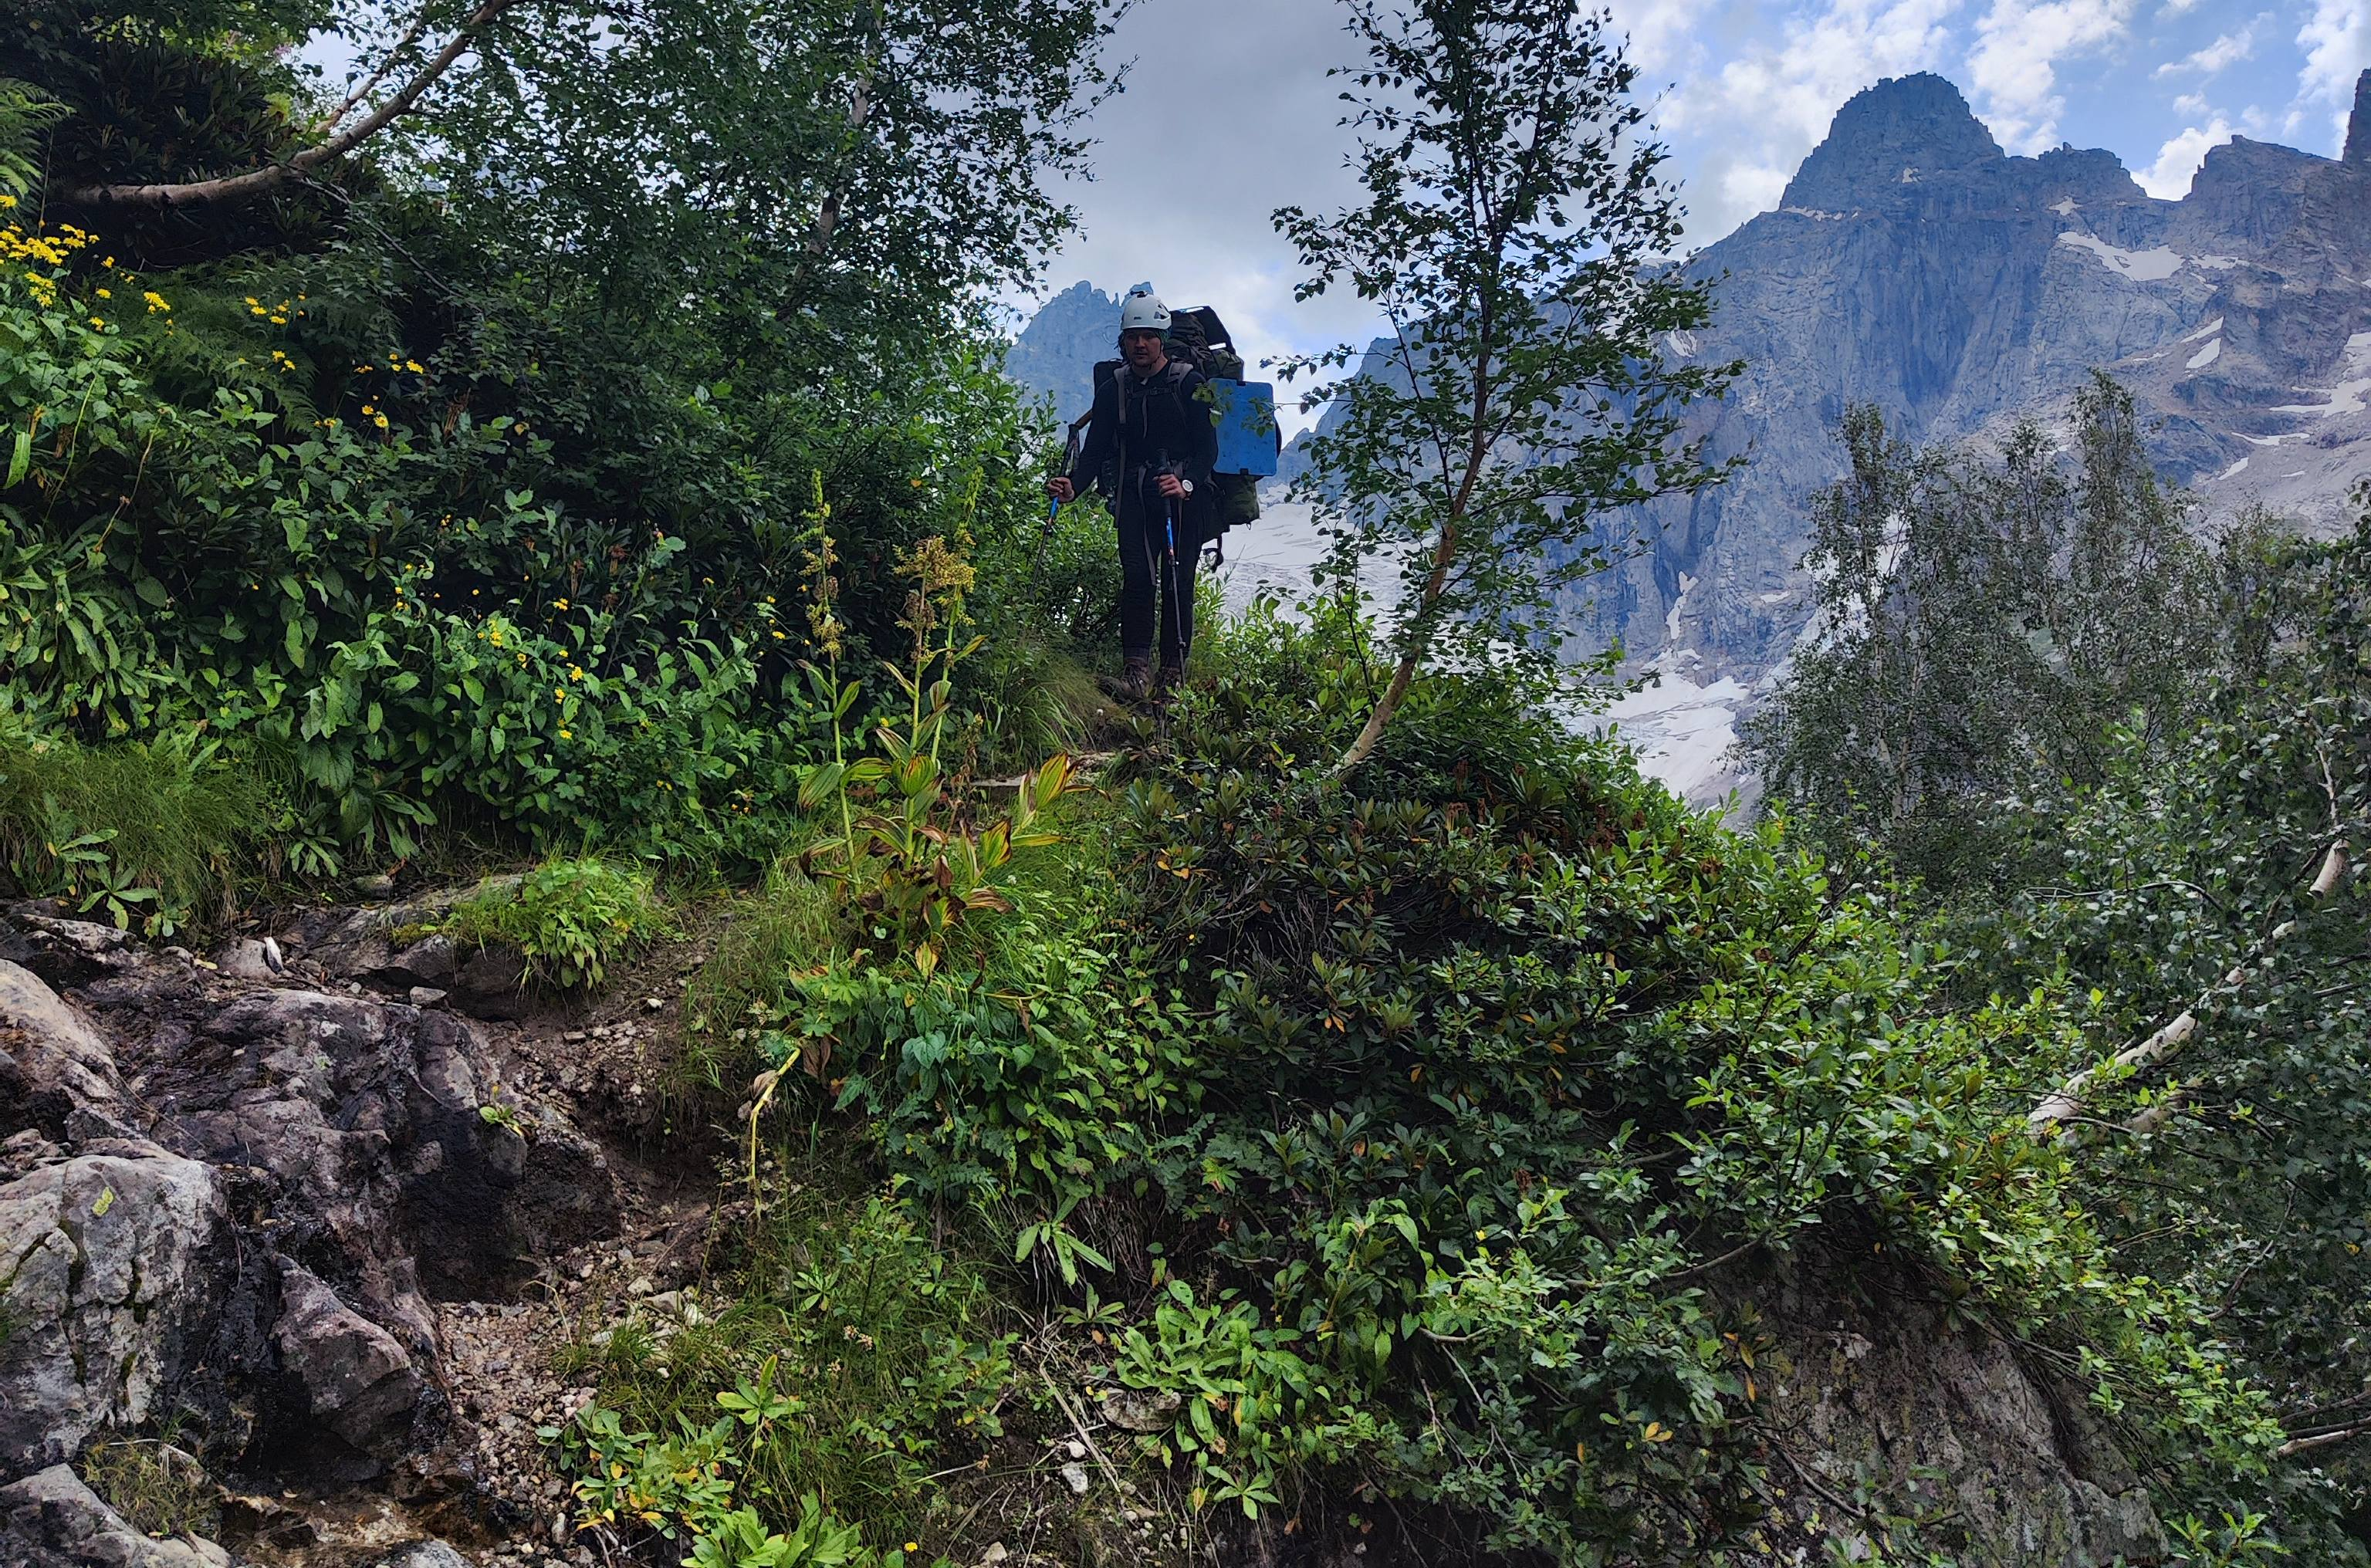
\includegraphics[width=0.7\linewidth]{../pics/IMG_20240825_134744.jpg}
	\caption{Тропа по склону р. Кичкинекол к Таллычатским ночёвкам}
	\label{fig:IMG_20240825_134744.jpg}
\end{figure}


В 14:40 вышли из зоны леса к нижним Таллычатским ночёвкам. Нашему взору представились потрясающие виды на ГКХ (рис.~\ref{fig:DSC_0158.JPG}). 

\begin{figure}[h!]
	\centering
	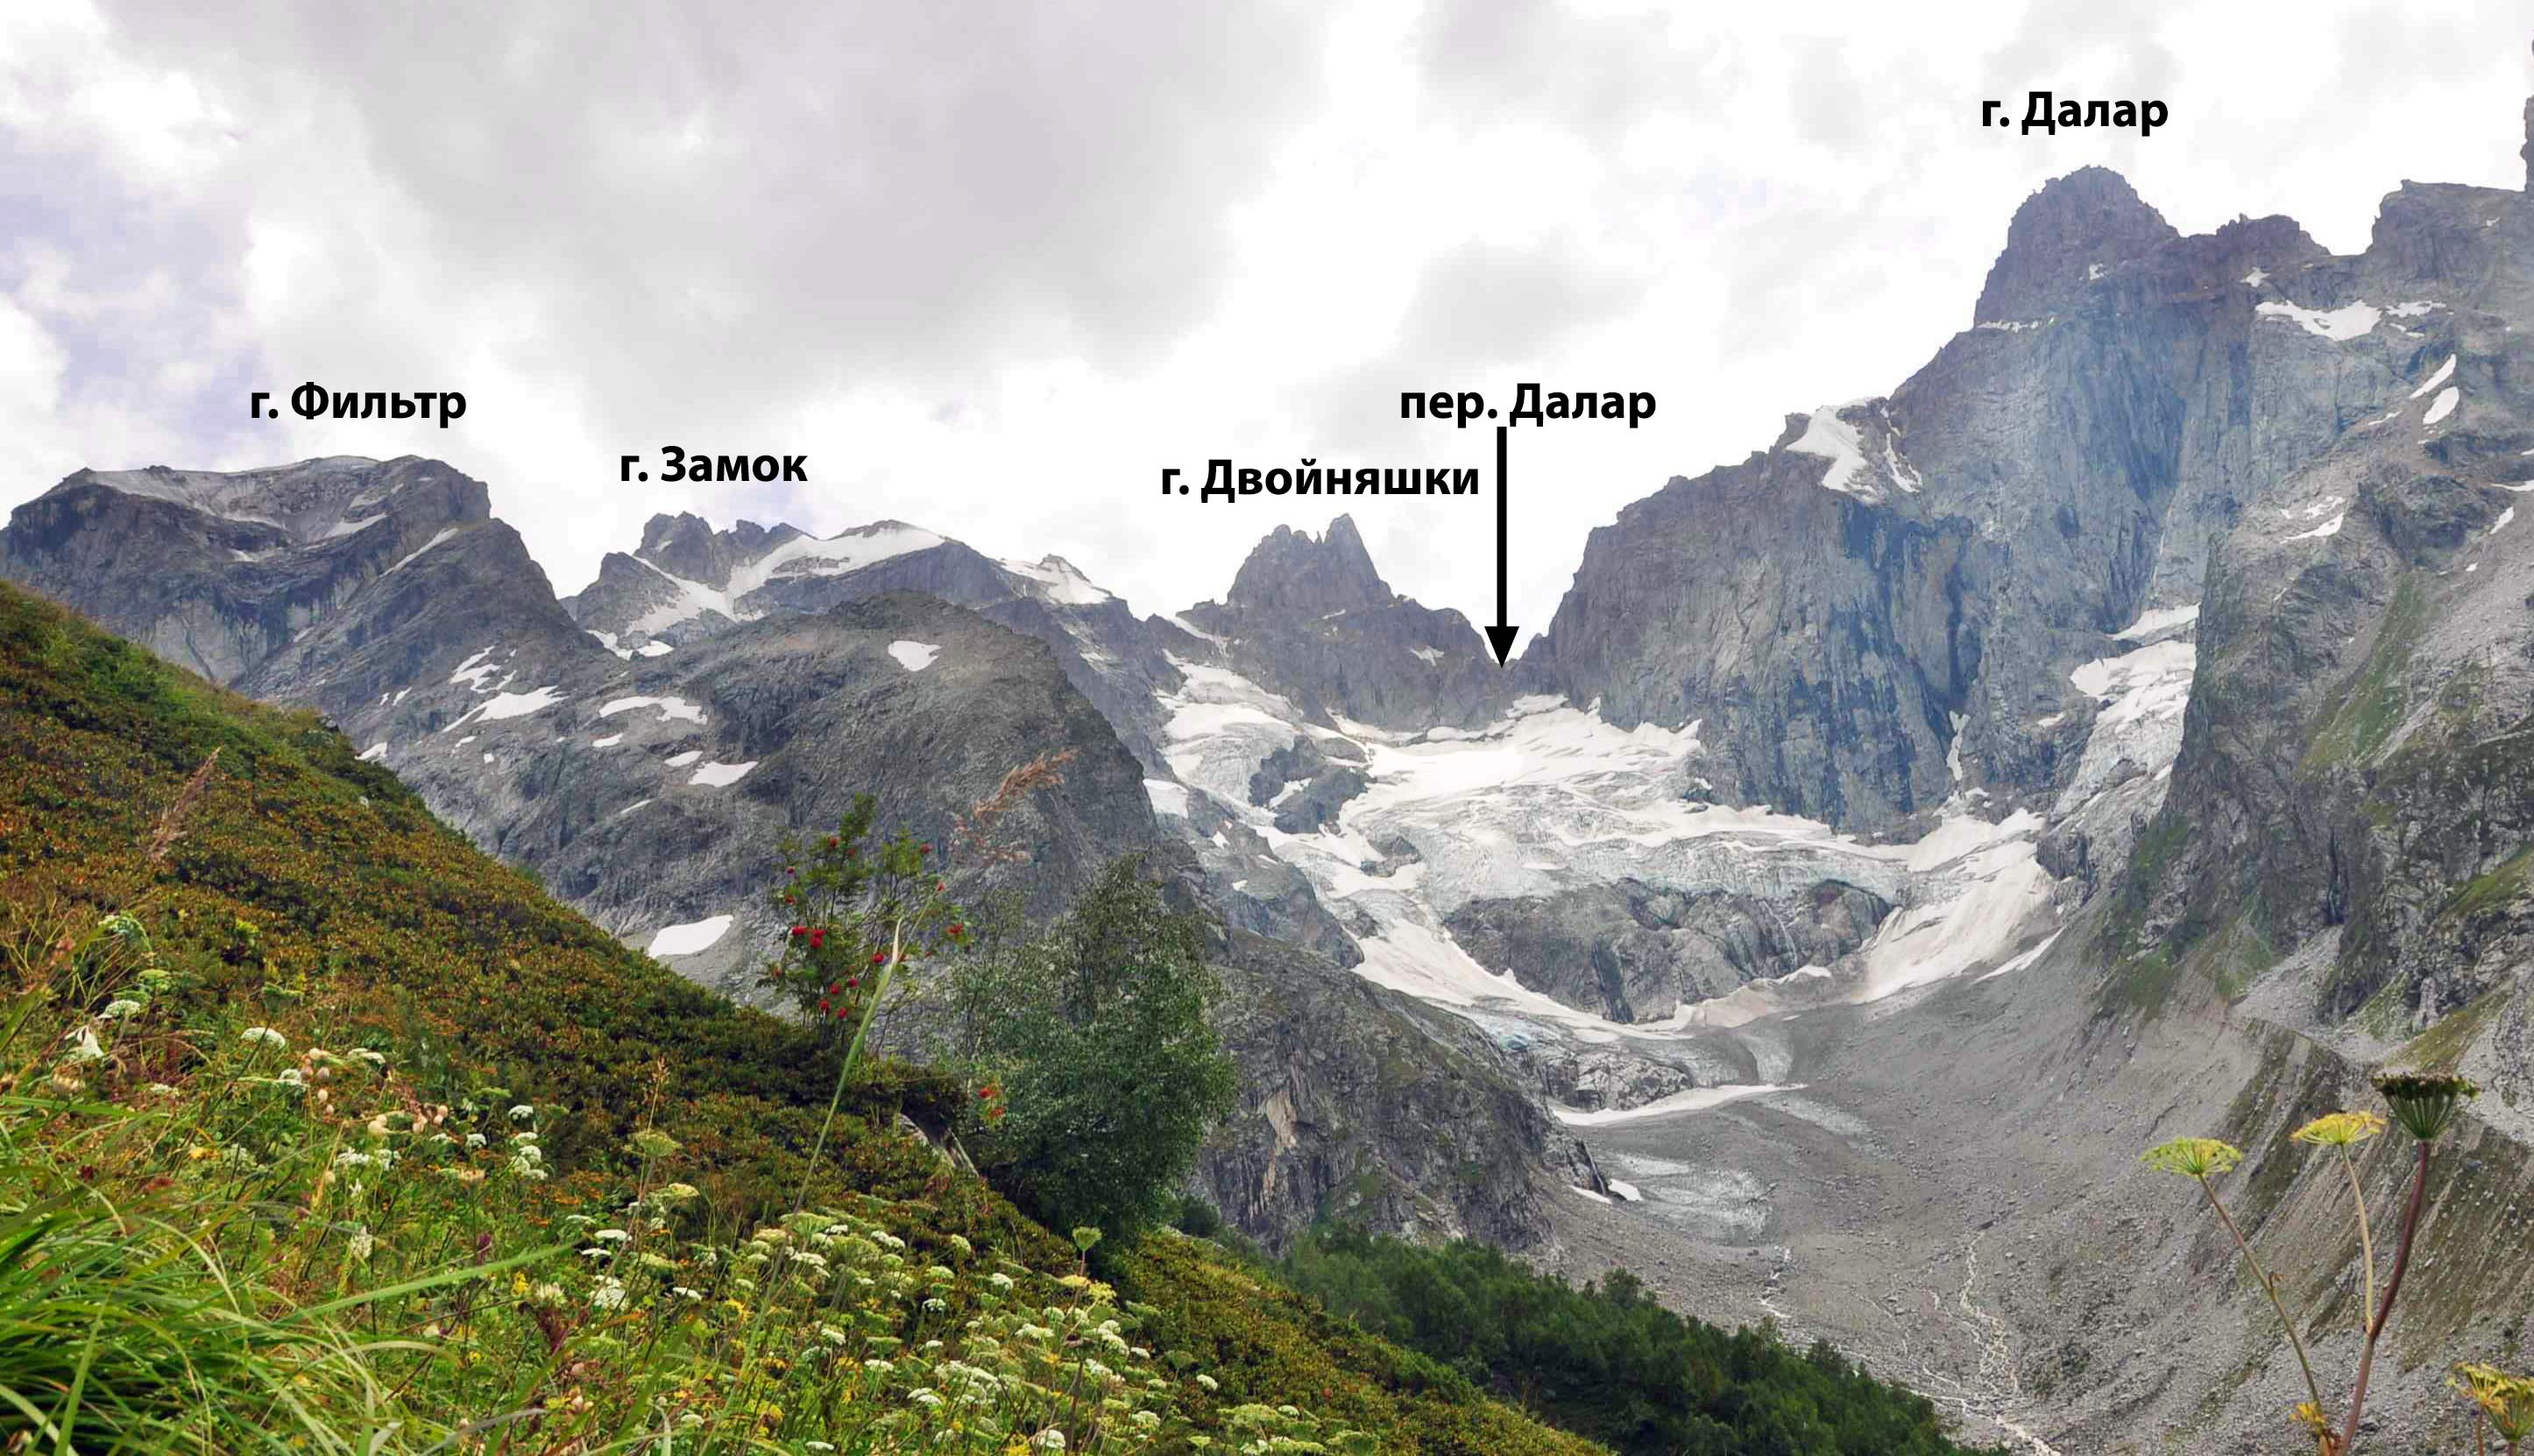
\includegraphics[width=0.7\linewidth]{../pics/DSC_0158.jpg}
	\caption{Вершины и перевалы ГКХ в районе пер. Кичкинекол}
	\label{fig:DSC_0158.JPG}
\end{figure}

Дальшейший путь до м.н. не представлял особого труда, если не учитывать красивые виды вокруг и обилие шикши под ногами.

В 16:04 пришли на наше м.н., пересохшее озеро, которое называется сейчас Поляной Крокусов. Поставили  палатки, при начинающемся дожде приготовили ужин, и сразу после этого дождь перешёл в ливень, а затем разразилась гроза. Непогода не прекращалась до часу ночи, некоторые участники были вынуждены рыть дренажные канавы, чтобы не затапливало палатки. Утром мы порадовались, что встали в верхней части стоянок, так как нижняя часть озера за ночь перестала быть пересохшей.
Координаты м.н. N43.249638\degree, E42.198292\degree.

\begin{figure}[h!]
	\centering
	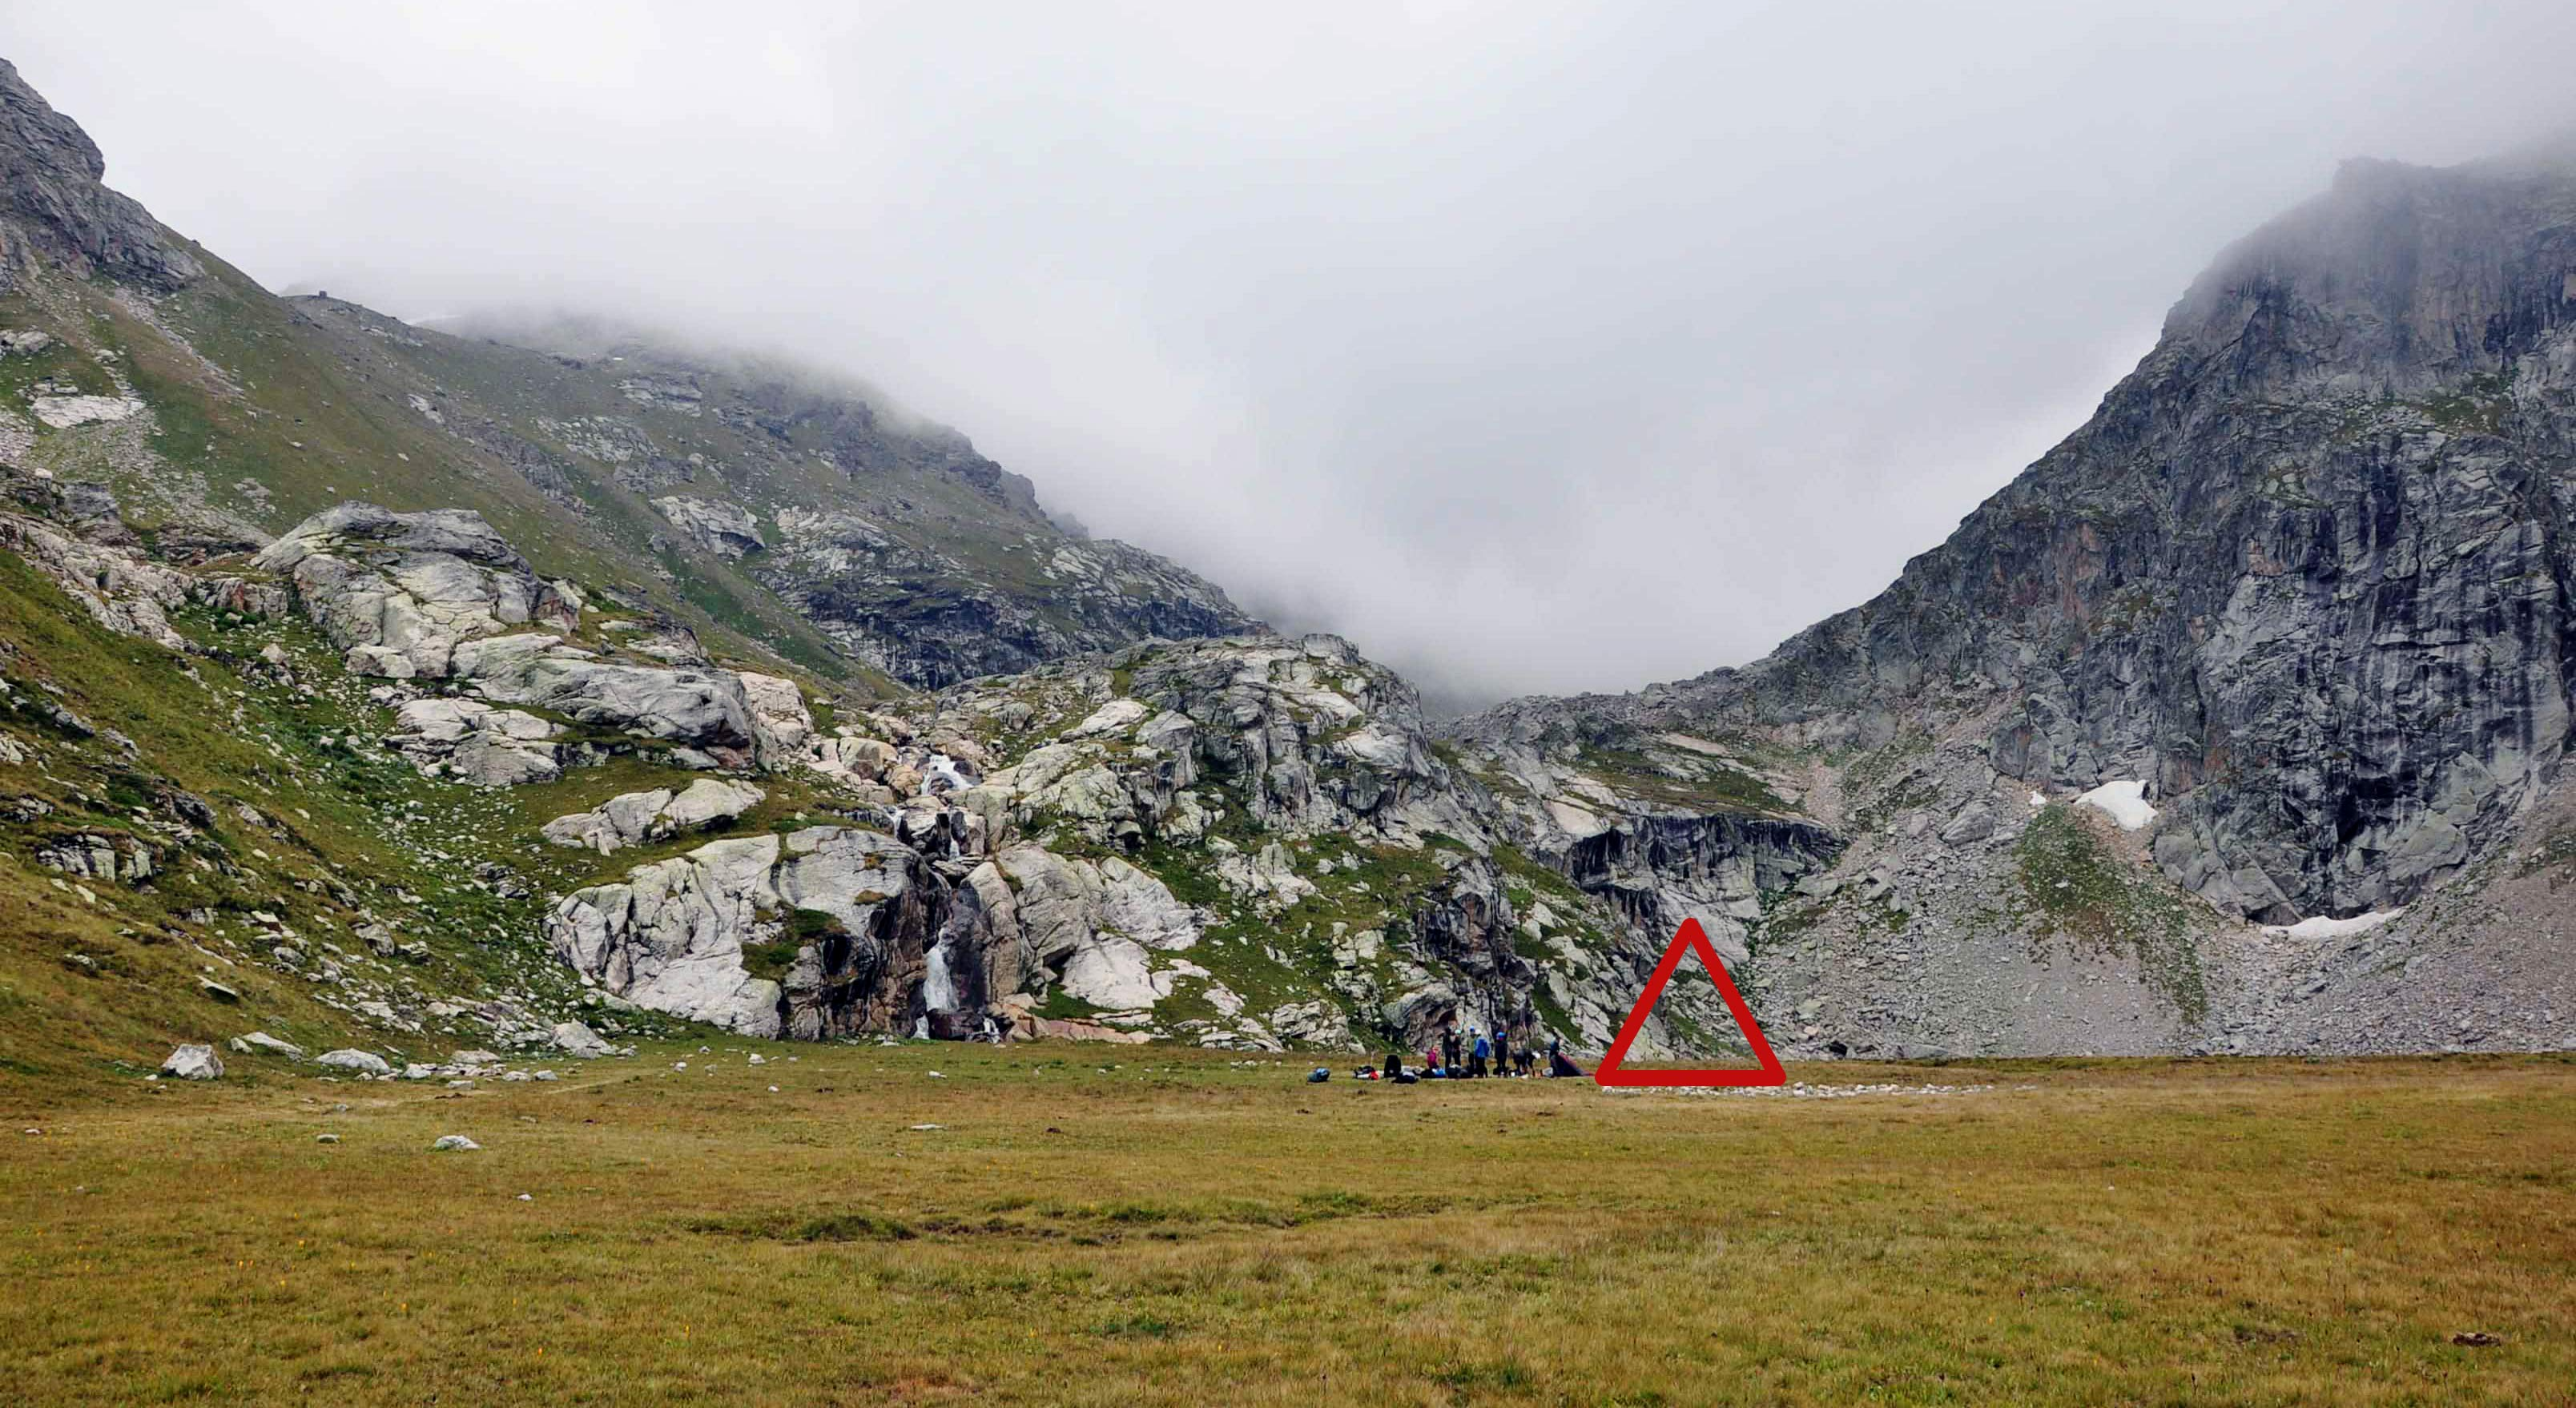
\includegraphics[width=0.7\linewidth]{../pics/DSC_0177.jpg}
	\caption{м.н. 25-26 августа}
	\label{fig:DSC_0177.JPG}
\end{figure}


\clearpage